\section{Implementação e Análise}
    \label{sec:exp}
A implementação foi realizada em Python, ver. $3.7.6$, está disponível online no~\hyperlink{https://github.com/rodrigofegui/IA-proj1}{GitHub} e foi modularizada em quatro arquivos:~\texttt{variables},~\texttt{utils},~\texttt{genetic\_algorithm} e~\texttt{main}, com relacionamento demonstrado na Figura~\ref{fig:exp_arqs}.

As constantes controlam o contorno do algoritmo genético, podendo alterar seu comportamento, tais como: $\mathbf{population\_sz}$ é o tamanho da população, $\mathbf{crossover\_pbty}$ é a probabilidade de combinação, $\mathbf{mutation\_pbty}$ é a probabilidade de mutação, $\mathbf{current\_indv\_perc}$ é a porcentagem da geração atual a ser mantida na próxima geração, $\mathbf{stability\_perc}$ é a porcentagem para ser considerável como estável e $\mathbf{stability\_max}$ é a quantidade máxima de gerações a serem consideradas estáveis. Além disso, alguns trechos de código serão explicados:

\begin{itemize}
    \item \textbf{etapas do algoritmo genético:} conforme demonstrado no Código~\ref{cod:etapas}, a população é ordenada considerando sua adaptabilidade ao ambiente, caso a estabilidade for atingida, o algoritmo é interrompido, caso contrário novos indivíduos são gerados a partir da combinação e da mutação da geração corrente;
    \item \textbf{combinação de cromossomos}: conforme demonstrado no Código~\ref{cod:combinacao}, toda a geração é considerada como prováveis pais, mas os com adaptabilidade semelhantes formarão pares. Caso a probabilidade de combinação não tenha sido atingida, o par é ignorado, caso contrário um dos quatro tipos de combinação disponível é selecionado para o par.
\end{itemize}

\begin{figure}[!h]
    \centering
    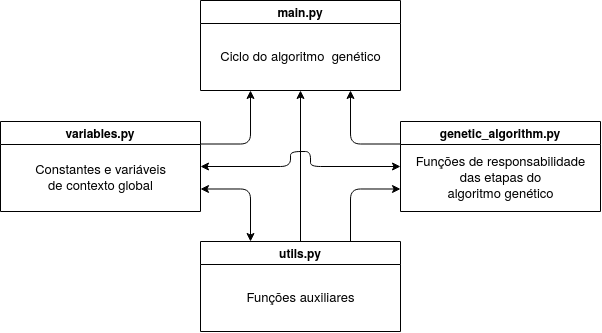
\includegraphics[width=\linewidth]{Imagens/Implementação_Diagrama.png}
    \caption{Relacionamento entre os arquivos da implementação.}
    \label{fig:exp_arqs}
\end{figure}

\begin{lstlisting}[float, floatplacement=H, caption={Trecho da implementação das etapas do algoritmo genético.}, label={cod:etapas}, language=Python]
for cnt in range(GENERATION_MAX):
    generation = fitness(generation)

    if reached_stability(generation):
        break

    new_individuals = crossover(
        generation
    )
    new_individuals.extend(
        mutation(generation)
    )
\end{lstlisting}

\begin{lstlisting}[float, floatplacement=H, caption={Combinação de dois cromossomos.}, label={cod:combinacao}, language=Python]
def crossover(generation):
    new_individuals = []
    options = [
        _crossover_order1,
        _ordered_crossover,
        _uniform_crossover,
        _crossover_2_point
    ]
    
    for ind in range(0,len(generation),2):
        if random() > CROSSOVER_PBTY:
            continue
    
        new_individuals.extend(
            choice(options)(
                generation[ind],
                generation[ind + 1]
            )
        )
    
    return new_individuals
\end{lstlisting}

Devido à sua natureza aleatória e baseada no evolucionismo, o algoritmo genético não terá o mesmo comportamento a cada geração para o mesmo conjunto de parâmetros, uma vez que a Figura~\ref{fig:exp_best} encontrou a menor distância, $128$, em poucas gerações, $88$, enquanto que pela Figura~\ref{fig:exp_worst} não foi encontrado a menor distância, obtendo $144$, e utilizou todas as gerações possíveis; considerando os seguintes parâmetros iniciais: $\mathbf{population\_sz}=40$, $\mathbf{crossover\_pbty}=0.78$, $\mathbf{mutation\_pbty}=0.1$, $\mathbf{current\_indv\_perc}=0.6$, $\mathbf{stability\_perc}=0.1$ e $\mathbf{stability\_max}=10$.

Utilizando o algoritmo com as constantes iniciais mencionadas anteriormente, foram encontradas, em algumas execuções do algoritmo, duas rotas para a distância mínima de 128: \textbf{Brasília -> Caracas -> Bogotá -> Lima -> Santiago -> Salvador -> Porto Alegre -> São Paulo -> Rio de Janeiro -> Belo Horizonte -> Brasília}, e \textbf{Brasília -> Belo Horizonte -> Rio de Janeiro -> São Paulo -> Porto Alegre -> Salvador -> Santiago -> Lima -> Bogotá -> Caracas -> Brasília}.

\begin{figure}[!h]
    \centering
    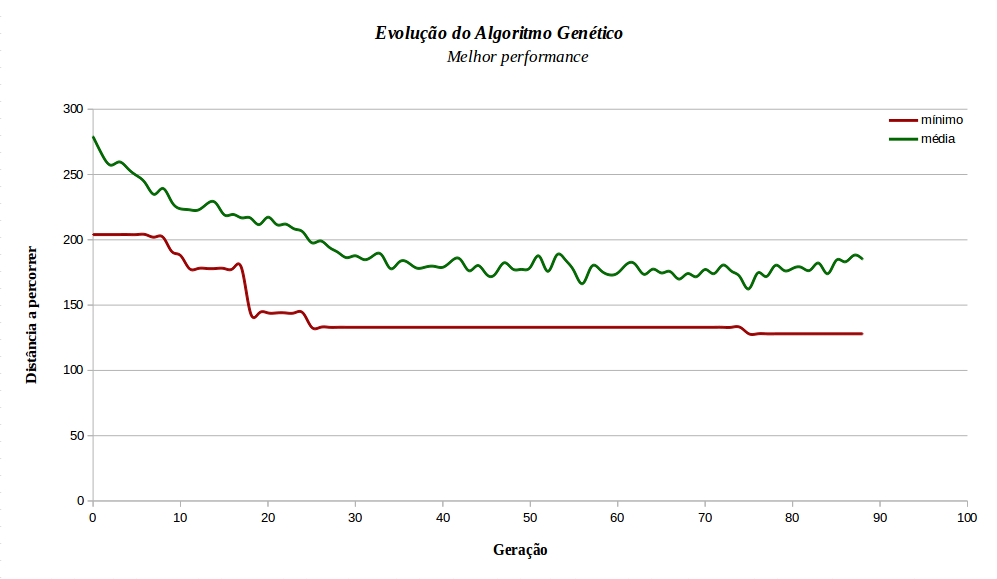
\includegraphics[width=\linewidth]{Imagens/best_perfomance.png}
    \caption{Um dos melhores comportamentos do algoritmo genético.}
    \label{fig:exp_best}
\end{figure}

\begin{figure}[!h]
    \centering
    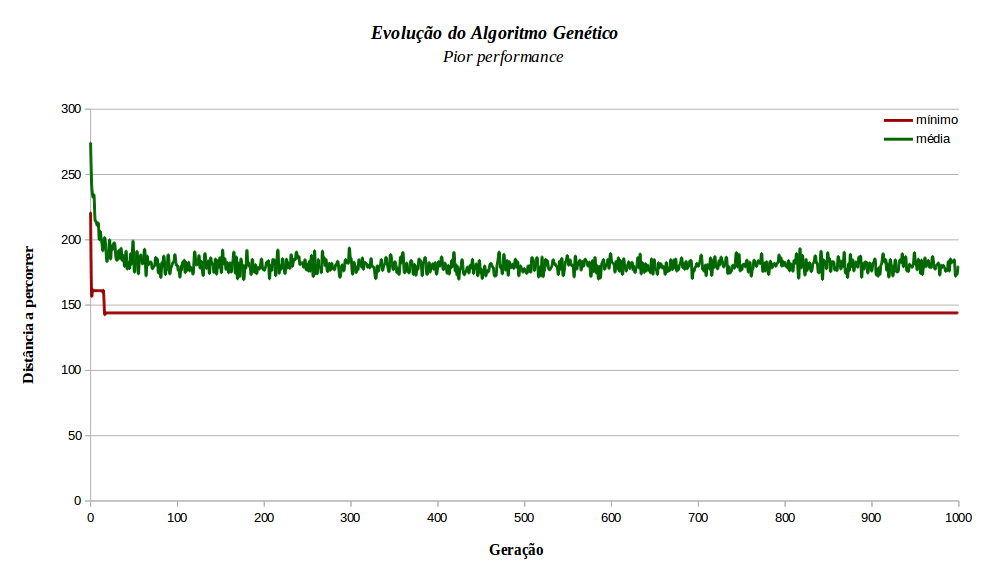
\includegraphics[width=\linewidth]{Imagens/worst_performance.png}
    \caption{Um comportamento mediano do algoritmo genético.}
    \label{fig:exp_worst}
\end{figure}


Com a finalidade de analisar o comportamento do algoritmo ao alterar alguns de seus parâmetros de contorno, foram realizadas modificações nos valores iniciais das constantes $\mathbf{population\_sz}$, $\mathbf{current\_indv\_perc}$, $\mathbf{crossover\_pbty}$ e $\mathbf{mutation\_pbty}$.

Na Figura~\ref{fig:exp_sz_populacao}, foi alterada a constante $\mathbf{population\_sz}$ de $40$ para $200$. Com isso, observa-se que a média da distância a percorrer decai de forma mais suave, sem apresentar variações bruscas e, assim, atinge o intervalo de estabilidade em poucas gerações. Além disso, o algoritmo consegue atingir a distância mínima de 128 dentro do número de gerações até a estabilidade.

Na Figura~\ref{fig:exp_perc_elitismo}, foi reduzida a constante $\mathbf{current\_indv\_perc}$ de $0.6$ para $0.1$. Verificou-se que o algoritmo apresentou uma média da distância a percorrer mais elevada (acima de 200) e instável, o que levou a mais gerações até a estabilidade. Entretanto, ainda foi possível atingir a distância mínima de 128.

Na Figura~\ref{fig:exp_prob_combinacao}, a constante $\mathbf{crossover\_pbty}$ foi reduzida de $0.78$ para $0.1$. Observou-se que embora a distância mínima de 128 foi atingida em menos de 200 gerações, a menor porcentagem de cruzamento tornou a média da distância a percorrer mais instável e o algoritmo foi levado até o número máximo de $1000$ gerações.

Por fim, na Figura~\ref{fig:exp_prob_mutacao}, a constante $\mathbf{mutation\_pbty}$ sofreu aumento de $0.1$ para $0.3$. Com essa alteração, observou-se que a distância mínima foi atingida por volta da 50\textsuperscript{\d a} geração. Esse valor baixo de gerações até encontrar a distância mínima pode ser explicado pelo fato de não haver genes repetidos em um indivíduo, o que pode tornar a mutação mais eficiente. Por outro lado, o algoritmo percorreu $250$ gerações até atingir a estabilidade, pois a média da distância a percorrer ainda apresentou variação considerável.

\begin{figure}[!h]
    \centering
    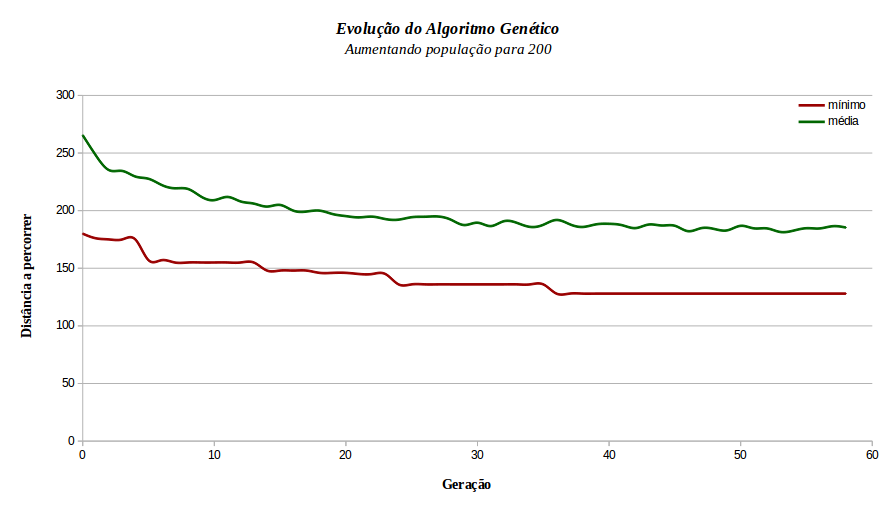
\includegraphics[width=\linewidth]{Imagens/sz_populacao=200.png}
    \caption{Comportamento aumentando o tamanho da população de 40 para 200.}
    \label{fig:exp_sz_populacao}
\end{figure}

\begin{figure}[!h]
    \centering
    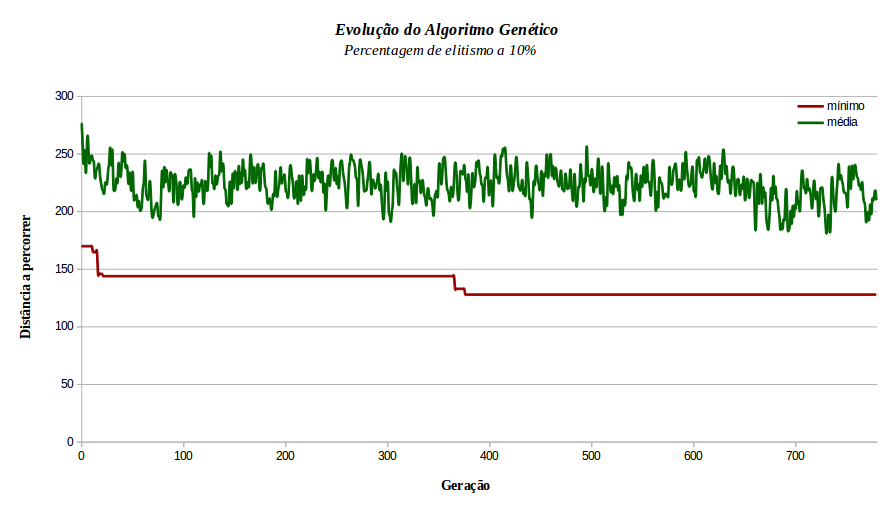
\includegraphics[width=\linewidth]{Imagens/perc_elitismo=10.png}
    \caption{Comportamento ao reduzir a porcentagem da geração atual a ser mantida para a próxima geração de 0.6 para 0.1.}
    \label{fig:exp_perc_elitismo}
\end{figure}

\begin{figure}[!h]
    \centering
    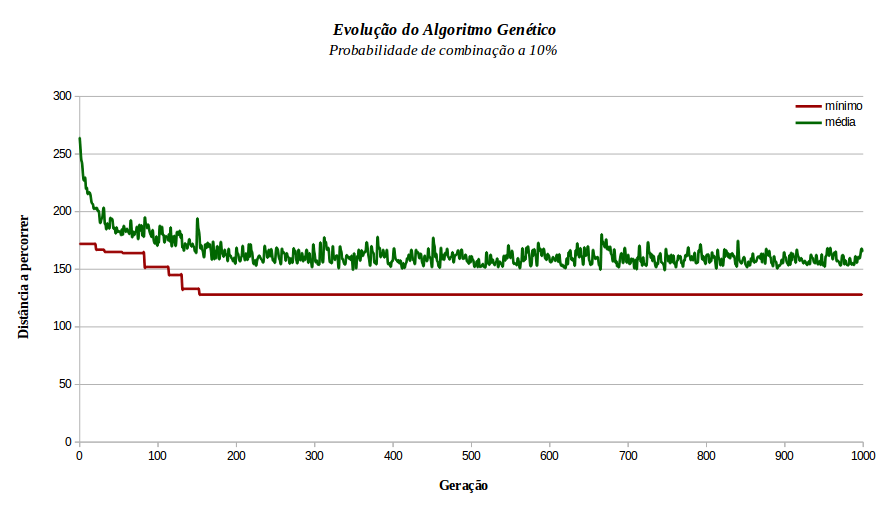
\includegraphics[width=\linewidth]{Imagens/prob_combinacao=10.png}
    \caption{Comportamento ao reduzir a probabilidade de combinação de 0.78 para 0.10.}
    \label{fig:exp_prob_combinacao}
\end{figure}

\begin{figure}[!h]
    \centering
    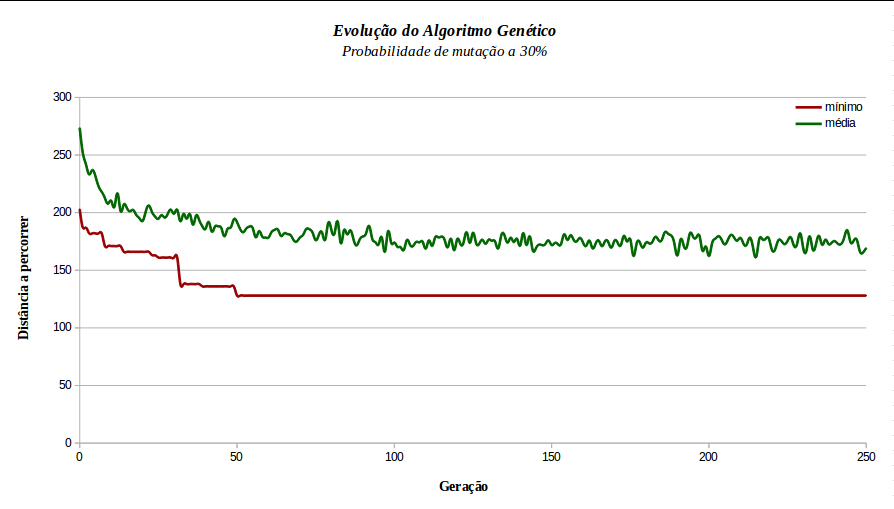
\includegraphics[width=\linewidth]{Imagens/prob_mutacao=30.png}
    \caption{Comportamento ao aumentar a probabilidade de mutação de 0.1 para 0.3.}
    \label{fig:exp_prob_mutacao}
\end{figure}